\chapter{Deep Networks for CFO}

\section{Recurrent Neural Network Follows a Circle}

We first explore what kind of architectures are necessary for a recurrent neural network (RNN) to learn how to follow a circle.
We show that a simple, small linear RNN can learn to act as the rotation matrix for a single rate of rotation around a circle.
We also show that in order to have an RNN follow a circle for different rates of rotation, we need a large non-linear layer.

\subsection{Single Rate}

\setlength{\tabcolsep}{0pt}
\begin{figure}
  \centering
  \caption{Linear neural network: follow a circle for a constant CFO rate.}
  \begin{tabular}{ccc}
    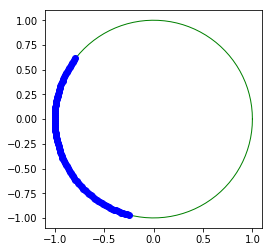
\includegraphics[width=50mm]{figures/cfo/follow_circle_linear_before.png}&
    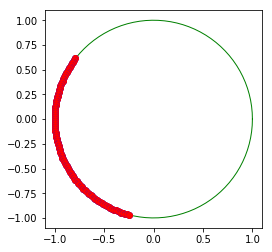
\includegraphics[width=50mm]{figures/cfo/follow_circle_linear_after.png}&
    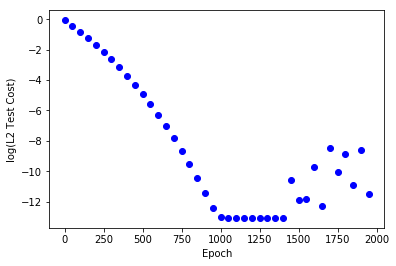
\includegraphics[width=70mm]{figures/cfo/follow_circle_linear_loss.png}\\
  \end{tabular}
  \label{fig:circle_constant_rate}
\end{figure}

Figure~\ref{fig:circle_constant_rate} shows a recurrent neural network (RNN) that follows a circle for a single rate of rotation.  The network's input is the starting point, $x[0]$, and it must predict the next $100$ points, $x[1] \ldots x[99]$.  Point $x[i]$ is rotated by $e^{ij\omega}$ where $\omega$ is the rate of rotation.  The RNN architecture is one linear layer that takes the current point as input, $x[i]$, and outputs the next point, $x[i+1]$.  We are forcing the state of the RNN to be the next point; $\text{state} = x[i+1]$.  We use a linear layer here because the network essentially has to learn how to become the rotation matrix which is linear with respect to the input. 

\begin{align}
R = \begin{bmatrix}
\cos(\omega) & - \sin(\omega) \\
\sin(\omega) & \cos(\omega)
\end{bmatrix}
\end{align} 

The RNN was trained for a constant rate of rotation, $\omega$, applied to sequences of $100$ points.  The network trained for $2k$ epochs, each with a batch size of $1k$ data sequences and with a learning rate of $0.006$.  The initial starting point, $x[0]$ is a uniform random variable drawn from on the unit circle. 
The network is tested on $1k$ new data sequences but with the same $\omega$.
Figure~\ref{fig:circle_constant_rate} shows the results of an RNN trained and tested for $\omega=0.02$.  The network achieves a loss on the order of $10^{-13}$.  

\subsection{Different Rates}

\setlength{\tabcolsep}{0pt}
\begin{figure}
  \centering
  \caption{Nonlinear neural network: follow a circle for a different CFO rates.}
  \begin{tabular}{ccc}
    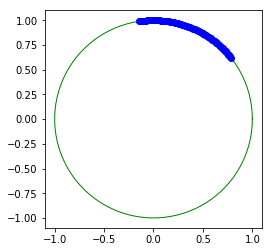
\includegraphics[width=50mm]{figures/cfo/follow_circle_nonlinear_before.png}&
    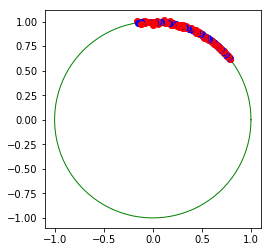
\includegraphics[width=50mm]{figures/cfo/follow_circle_nonlinear_after.png}&
    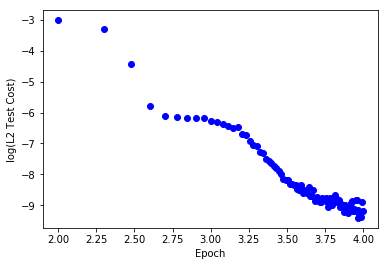
\includegraphics[width=70mm]{figures/cfo/follow_circle_nonlinear_loss.png}\\
  \end{tabular}
  \label{fig:circle_diff_rate}
\end{figure}

Figure~\ref{fig:circle_diff_rate} shows a recurrent neural network (RNN) that follows a circle for a given rate of rotation.
The network's input is the starting point, $x_0$ and the rate of rotation, $\omega$.
The RNN must predict the next $100$ points, $x_1 \ldots x_{99}$.  Point $x_i$ is rotated by $e^{ij\omega}$.

We cannot use just linear layers in this case because the RNN must learn to find $\cos(\omega)$ and $\sin(\omega)$ for different $\omega$.  Essentially, this RNN needs to approximate the $\sin, \cos$ functions an then apply them to the data points.

The RNN architecture consists of one non-linear layer, with $100$ nodes and Relu activation functions, and a linear layer at the output with $2$ nodes. The input to the RNN is the estimated current point, $\hat{x}_i$, and the rate of rotation, $\omega$.  The RNN outputs the estimate of the next point, $\hat{x}_{i+1}$.  We are forcing the state of the RNN to be the estimate of the next point concatenated with the rate of rotation; $\text{state} = [\hat{x}_{i+1},\omega]$ so that state then becomes the input to the next run of the RNN.

The RNN is trained for different rates of rotation, $\omega$, applied to sequences of $100$ points.
The rate of rotation is a uniform random variable drawn from $0-\frac{1}{50}$.
We use mean squared error of the true data sequence and the estimated data sequence for the loss function; $||\vec{x}-\vec{\hat{x}}||^2$.  The network is trained for $10k$ epochs, each with a batch size of $1k$ data sequences and with a learning rate of $0.01$.  The initial starting point, $x_0$ is a uniform random variable drawn from on the unit circle.
The network is tested on $100k$ new data sequences with random $\omega$.
Figure~\ref{fig:circle_constant_rate} shows the results of an RNN trained and tested for $10k$ epochs.  The network achieves a loss on the order of $10^{-5}$.


\section{Deep Network Carrier Frequency Offset Estimation}
\begin{itemize}
\item complex gradients problems
\item act like the real and imaginary parts are separate
\item plots: one tap channel plots, without equalization problems
\item plots: two tap channel plots, with equalization problems
\end{itemize}

\begin{figure}
\begin{center}
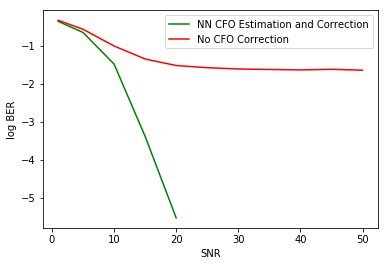
\includegraphics[width=12cm]{figures/cfo/cfo_estimation.png}
\caption{The log BER of received signals passed through a neural network CFO estimator with a rotation matrix CFO correction and classic demodulator. The log BER of the same signals passed through just the classic demodulator.}
\label{fig:cfo_est}
\end{center}
\end{figure}

Figure~\ref{fig:cfo_est} shows how...

%\section{Deep Network Carrier Frequency Offset Correction}
%Program a Costas loop for comparison 